\section{Speech Processing software and tools}
\subsection{Alisa}\label{c3sec_alisa}
Alisa tool is a lightly supervised sentence segmentation tool based on Voice Activity Detection (VAD) algorithms \citep{stan2016alisa}.  It is so called lightly supervised because it requires small amounts of training data.  Generally the tool was asserted to be optimised for sentence segmentation and offered assistance in the creation of new speech corpora in a language-independent fashion. 

The Alisa tool researchers deploy a two-step method for aligning speech, and claim performance up to 70\% imperfect transcriptions often found in online resources can be successfully aligned with a word error rate of less than 0.5\%.  This tool is therefore said to be suitable for development multilingual and under-resourced language aligned speech-corpora.

The motivation behind Alisa was to reduce the time and effort used to gather a large amount of large amounts of quality data as well as actively eliminate the domain knowledge required to phonetically transcribe speech data.  In addition, and as a bonus to achieving the first objective, is the ability to migrate speech technology fairly seamlessly from one language to another and therefore realise the rather tedious task of automatic transcription of a new language.

\subsubsection{Alisa Architecture}
The goal of automatic transcription of new language with low resource constraint is particularly valuable to this research and as such, it would be relevant to review the enhancements introduced to Alisa.  The two step-method consists of a GMM-based sentence level segmenter and also an iterative grapheme acoustic model used for alignment.  The sentence level GMM-based speech segmenter is used to automatically segment speech into utterances which as discussed earlier forms the basic unit of processing within any ASR system.  This attempts to relieve the researcher off the manual process of segmenting the continuous audio file manually. This process included a GMM-based voice activity detector trained from about 10 minutes of manually labeled data. The second step grapheme based acoustic model is supplemented with a highly restricted word network they referred to as a skip network.  Together an iterative acoustic modelling training procedure is formulated.  The method described required the initial training data and a minimal labelling procedure that involved simple letter to sound rules and inter-sentence silence segments to provide an orthographic transcript of the initial 10 minute recording data.  Therefore, this process is resource-effective because non-experts can also provide this data.  The actual alignment process made use of a grapheme level Viterbi decoder to drive the iteratively self-trained grapheme models.  The model architecture is shown in the figure below.
\begin{figure}
\centering
  % Requires \usepackage{graphicx}
  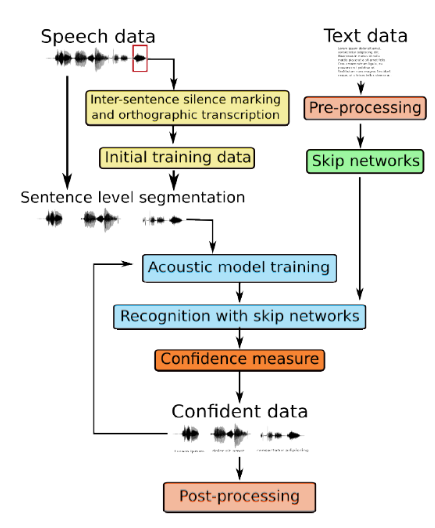
\includegraphics[width=9cm]{thesis/images/alisa}\\
  \caption{Original waveform input for auto-correlation}\label{fig_c3_alisa00}
\end{figure}

Figure 3-5 Alisa Overview (Stan et al., 2016)
Figure 3-5 above shows a block diagram of the steps involved in the alignment.  The method can be applied to any language with an alphabetic writing system, given the availability of speech resource and its corresponding approximate script.

We have earlier mentioned that the downside of using grapheme based acoustic model is the increase in the error margin or trade of accuracy.  Several steps were introduced in Alisa to minimise this margin, the chief being the introduction of a tri-grapheme acoustic model which is modeled after using context dependent triphones in traditional acoustic modelling.  Other methods used drop down the error margin include the use of discriminative training with the Maximum Mutual Information (MMI) criterion (Schluter & Ney, 2001; Bouchard & Triggs, 2004) and methods described in (Novotney & Schwartz, 2009; Lamel, Gauvain & Adda, 2002). Finally, it was observed that Alisa provided good alignment but was not fully featured. For instance it had no way of adding insertions and substitutions in the audio data not provided in the transcription.  Secondly, Alisa is restricted to languages that can utilise the english alphabet.

\section{Initial Experiments}
The experiments in the following sections describe initial experiments based on the initial study of a language learning companion before the research was narrowed down to a low resource speech recognition.  These preliminary experiments in addition to a preliminary Language Learning Survey helped to narrow down the Research to the specific speech processing task of Low Resource Automatic Speech Recognition (LR-ASR).

The following sections describe analysis of raw wave-forms using auto-correlation signal processing in Matlab and experiments made with the Nao robot speech processing engine and experiments with speech recognition toolkit and speech processing tasks.  These tasks include digit recognition systems using CMUSphinx and Kaldi speech recognition toolkits and speech alignment tasks using Alisa tool.

\subsection{Auto-correlation Experiments}
Preliminary experiments were carried out on raw speech signals in an attempt to quickly segment individual phonemes based on a basic threshold algorithm.  Further experiments designed an autocorrelation algorithm to attempt to discover a phoneme alphabets in a particular dataset in a semi-supervised fashion.
 
This method had desirable goals when compared with other segmentation techniques outlined in the previous chapter. The chief being the ability to simulate a posterior distribution statistic from auto-correlation estimate.  This presents an unnormalised posterior distribution measurement of every phoneme segments over the entire signal.

The correlation theory is based on the idea that when a signals is superimposed on itself in a time-shifted manner, the convolution over itself is highest when the two signals have zero time lag that is, perfectly overlapped in sync and the better the overlapping the higher the value of the correlation and the lesser the signals are matched they tend to cancel out each other and hence a very low value of the correlation.  The normalised auto-correlation value is obtained in \cite{picone1996fundamentals} from a signal $x(n)$ in the following equation:
\begin{equation}
    \Psi(i)=\frac{\sum_{n=0}^{N-1}x(n)x(n-i)}{\left(\sum_{n=0}^{N-1}x(n)^2\right)\left(\sum_{n=0}^{N-1}x(n-i)^2\right)}\label{c3eq_corr}
\end{equation}
Based on experimental procedure, estimated locations of similar wave-forms representing segmented phonemes are calculated.  Although the procedure is subject to degrade in the face of most of the difficulties associated with dealing with raw audio waveform, it further emphasises the need for accurate speech features and pre-processing highlighted in the previous chapter.

This two stage procedure performs segmentation of phonemes and then discovery of phoneme clusters using a statistical auto-correlation algorithm.  The process is described in the following sections.
\begin{figure}
\centering
  % Requires \usepackage{graphicx}
  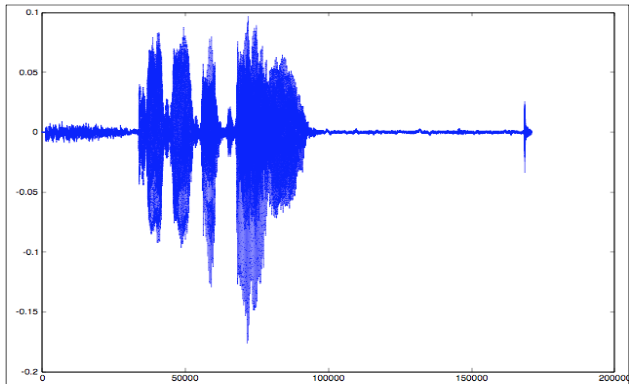
\includegraphics[width=9cm]{thesis/images/corr}\\
  \caption{Original waveform input for auto-correlation}\label{fig_c3_exp01}
\end{figure}

\subsubsection{Segmentation}
Figure \ref{fig_c3_exp02} describes the various steps of the segmentation phase while Figure \ref{fig_c3_exp01} shows the original audio file. At the segmentation phase, we first of all adjust the scale of the original raw audio file to have only positive values rather than having it centred on zero (Figure \ref{fig_c3_exp02}a).  At the next step a smoothing filter based on experimentation is used to perform both smoothing as well as determining the peaks and trough (Figure \ref{fig_c3_exp02}b).  Then a threshold is applied to segment the waveform based on discovered inflection points (Figure \ref{fig_c3_exp02}c).  
\begin{figure}
\centering
  % Requires \usepackage{graphicx}
  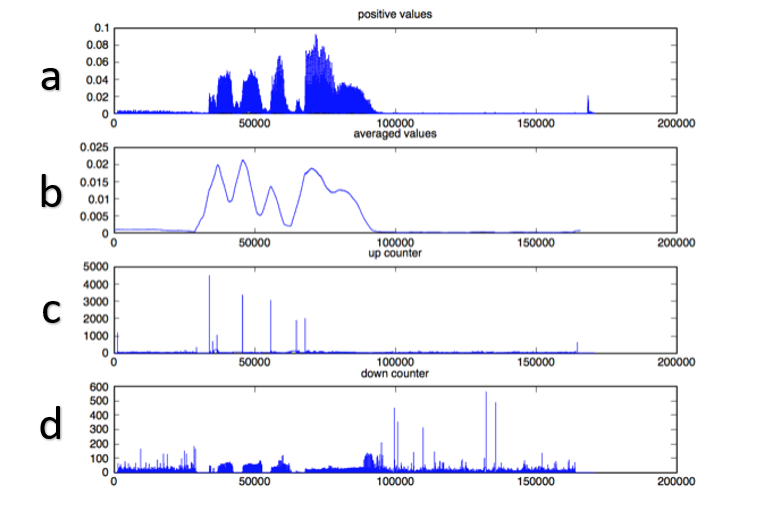
\includegraphics[width=9cm]{thesis/images/corr00}\\
  \caption{Original waveform input for auto-correlation}\label{fig_c3_exp02}
\end{figure}
\subsubsection{Auto-correlation}
At the auto-correlation stage estimated phoneme segment boundaries are stored in an array and cross-correlated with the original signal.  Even though at a top-level view, the entire signal is auto-correlated, at the individual segment level, the signals are cross correlated against one another.  Furthermore, to achieve a ‘fair’ correlation estimate, individual segments representing estimated phonemes need to be re-sampled to eliminate mismatching of contour representations of the individual phonemes.

The proposed auto-correlation algorithm performs both top-down and bottom-top processing.  In the first stage it does bottom-top segmentation, while in the second phase top-bottom auto-correlation.   The major weakness is this auto-correlation method the segmentation algorithm, data filtering and the feature representation.  The Bayesian method of segmentation \citep{kamper2016unsupervised} which is related to this method also improved on these weaknesses was able to improve on these weakness by using ASR feature preprocessing and a combination of acoustic embedding Dynamic Time Warping (DTW) for clustering rather than auto-correlation.  In effect using the extracted features for clustering is in theory a better speech estimate with less intrinsic noise for classification than using an only smoothed audio data.

\subsection{Experiments with Nao robot}
Nao is a humanoid robot developed mainly for deployment in environments for robotics education and development purposes.  Nao comes with a speech recognition software that offers features such as language settings and recognition sensitivity.  However it was understandably found to be limited because the Nao robot itself does not possess the processing power to perform CPU intensive training of acoustic models.  The now robot did however offer a level of support for using the pocketsphinx system. The pocketsphinx system is the C-language equivalent of CMUSphinx speech recognizer system also by Carnegie Mellon University.  Using the pocketsphinx method, acoustic models trained high performance systems can then be deployed to Nao for fast decoding within the Nao.  

\subsection{Digit Speech Recognition and Alignment Experiments}\label{sec_digitspeech}
These experiments were performed using CMU Sphinx4 recognition system and Kaldi speech recognition software.  While CMU Sphinx and pocketsphinx delivered standard interface for speech recognition using generative hybrid models, Kaldi speech in addition also offered advanced methods such as subspace Gaussian mixture model used to develop cross-lingual acoustic models and deep architectures for hybrid generative-discriminative models for speech recognition.   The main challenge with Kaldi was that it was CPU intensive and required a reasonable amount of parallel processing to achieve good results within a reasonable time period. 

Speech alignment experiments were performed using the Alisa \cite{stan2016alisa} tool which is a python based tool with calls made to the HMM toolkit \cite{young2002htk}.  The Alisa tool alignment process undergoes a semi-supervised process and requires an error prone time-intensive manual pre-alignment procedure.  The tool itself was found to be quite unstable and the output results were not very easily reproducible for further tests to be carried out on different datasets.  In addition to the time-intensive pre-alignment procedure made the tool not very useful for this research. Had the tool been more successful, the tool, which utilises Voice Activity Detection (VAD) algorithms, would have been especially useful for sentence segmentation of long sequences of transcribed audio speech.  This tool however still lacked in alignment at either a word-level or sub-word level of alignment required in ASR pipelines.


\section{End-to-end Research Experiments}\label{sec_postalign}
The main challenges of speech recognition using HMM-based toolkits such as Kaldi, is the requirement for aligned speech.  In more recent endeavours, there has been efforts towards automatic alignment of transcribed audio speech recordings through successive Baum-Welch estimation techniques \cite{gales2014speech,ragni2018automatic,ragni2014data}. However, this technique is not particularly compatible with end-to-end goals adopted for this research as it would require preprocessing and successive pre-training of the data set.

The following section describes the post-alignment experiments and in a later Chapter, how these methods deal with the problem of automatic speech alignment in a fashion which was compatible with end-to-end speech processing.  The end-to-end requirements were desirable for low-resource speech recognition as it introduces a simpler speech model design.  The downside however to the end-to-end approach is the dependency on very deep recurrent neural network structures which require large volumes of data for successful training.
\subsection{Tensor flow sequence-to-sequence character-to-diacritically-labelled-character model}\label{sec_c2d}
Experiments performed in this and the next three sections are all based on sequence-to-sequence modelling using recurrent neural networks. While the this and the following section represents precursor experiments around speech recognition tasks, the later two sections represent the final experiments reported in this work.

The character-to-diacritically labelled character model was a sequence-to-sequence diacritically labeled experiment to automatically infer diacritic transcriptions of the Wakirike language given the plain unmarked Wakirike language text as input.  This is a task, when achieved successfully is a sub task towards developing a phonetic dictionary for the Wakirike Language which in turn can be used in HMM speech recognition or equivalent  end-to-end models.  This experiment was a precursor experiment, the results of which were reserved for further study.
\subsection{Sequence-to-sequence Grapheme-to-Phoneme (G2P) model}
This is a follow up experiment to the previous experiment in section \ref{sec_c2d}. This model attempts to automatically generate a phonetic dictionary from graphemes in a text corpus. Grapheme-to-phoneme experiments come in two flavours. The first being a continuation of the previous experiment, that is, using diacritically marked symbols and the second flavour using non-marked graphemes as input.  The experiments we performed used the latter non-marked graphemes as input. As this experiment was also a subtask in HMM speech model building,  the results of these experiments were reserved for further study.  

What follows in the next three sections are sequence-to-sequence experiments actively developed in this research and are detailed in chapters (\ref{ch6_wlm,ch6_speech,ch8_future}).  A brief summary of the experiments are highlighted in the following sections (\ref{sec_grulm,sec_be2e,c3sec_espnet}).  Note that these models all utilise TensorFlow deep learning library including the Bi-directional speech model (section \ref{sec_be2e}) which is built on top of Mozilla DeepSpeech with the exception of section \ref{c3sec_espnet} which is based on pytorch; a similar deep learning library (see table \ref{tab_tfstats} for comparison).

\subsection{GRU language model for Wakirike language based on TensorFlow}\label{sec_grulm}
The language model developed in this research is a character-based sequence-to-sequence deep recurrent neural network that maps a sequence of characters to a sequence of words found in the training data set. This model met the objective of reducing the vocabulary size required for language models as well as the text corpus required as inferences could be made over the smaller-fixed character vocabulary rather than orders or magnitude larger word corpus with the possibility of out of vocabulary terms found in the training data.  Though this may occur in the character sequence-model at the inference stage.  It would not normally happen during training.  The neural network model developed is described in Chapters \ref{}, consists of Gated Recurrent Unit (GRU) Recurrent Neural Network (RNN). The GRU is a specialised type of Long Short-Term Memory (LSTM) cell RNN.  The emphasis here is on the ability to model over particularly long sequences of the training data.  In this case, over long character sequences.  Thus, the network is able to learn long term dependencies as would be naturally required to construct grammatically correct sentences.  In essence, the RNN is able to learn grammar rules inherently from the training data.

\subsection{Bi-Directional LSTM-based end-to-end speech model}\label{sec_be2e}
A similar LSTM sequence-to-sequence network based on Baidu Research’s original research design \citep{hannun2014deep} is developed in this research for end-to-end speech recognition.  This model, as its name implies, attempts to establish long term relationships by adding a reinforcing LSTM layer learning information but this time from the opposite direction, hence the bi-directional architecture.  

In addition, the model incorporates the Connectionist Temporal Classifier (CTC) decoder. This enables the model to make run-time inferences on both the character as well as estimate audio wave to character label alignment simultaneously.  This makes this design accommodate end-to-end goals and ultimately simplifies the overall design and completely eliminates the need for either manual or semi-supervised alignments mentioned previously in sections (\ref{sec_alisa,sec_digitspeech,sec_postalign}).

\subsection{ESP-Net Experiments}\label{c3sec_espnet}
The ESP-Net (End-to-end Speech Network) toolkit \citep{watanabe2018espnet}, is a speech processing toolkit that was of interest to this research because it offers end-to-end capabilities not only in Automatic Speech Recognition (ASR) but also in Text-To-Speech (TTS) or speech synthesis and other speech-sequence-processing related tasks.  In addition, the toolkit offered multi-modal training combining both Attention networks \cite{vaswani2017attention} with CTC networks as well as multi-channel feature representation that is, the fusing together of multiple feature representations of data.  Only preliminary experiments were carried out using ESPNet and is discussed in Chapter \ref{ch08furtherstudy} of this work.

\section{Method of evaluation}
System building methodology \citep{nunamaker1990systems} for speech recognition systems requires models to be evaluated against speech recognition Machine Learning metrics.  For language models, perplexity metric was used for evaluation.  Bleu has also been used as a metric for evaluating language models.

Perplexity measures the complexity of a language that the language model is designed to represent \citep{1976jelinekcontinuous}. In practice, the entropy of a language with an N-gram language model $P_N(W)$ is measured from a set of sentences and is defined as
\begin{equation}H=\sum_{\mathbf{W}\in\Omega}P_N(\mathbf{W})
\label{eqn_c2_lm05}
\end{equation}

where $\Omega$ is a set of sentences of the language. The perplexity, which is interpreted as the average word-branching factor, is defined as
\begin{equation}PP(W)=2^H
\label{eqn_c2_lm06}
\end{equation}
where H is the average entropy of the system or the average log probability defined as
\begin{equation}
H=-\frac{1}{N}\sum_{i=1}^N[log_2P(w_1,w_2\dots w_N)]
\label{eqn_c2_lm07}
\end{equation}
For a bi gram model therefore, equation (\ref{eqn_c2_lm07}) becomes
\begin{equation}
PP(W)=2^H=2^{-\frac{1}{N}\sum_{i=1}^N[log_2P(w_1,w_2\dots w_N)]}
\label{eqn_c2_lm08}
\end{equation}
After simplifying we have
\begin{equation}
PP(W)=\sqrt[N]{\prod_{i=1}^N\frac{1}{P(w_i|w_{i-1})}}
\label{eqn_c2_lm09}
\end{equation}


Full speech recognition pipelines are usually evaluated against the Word Error Rate (WER).  WER is computed as follows:
\begin{equation}\label{eqn_2_3_wer}
WER=\frac{I+D+R}{WC}\times 100
\end{equation}
Here $I,D,$ and $R$ are wrong insertions, deletions and replacements respectively and $WC$ is the word count.

Metrics used for low speech recognition in the zero speech challenge \citep{versteegh2015zero} include the ABX metric. Other common speech recognition error metrics following a similar definition as the Word Error Rate (WER) are Character Error Rate (CER), Phoneme Error Rate (PER) and Syllabic Error Rate (SyER) and sentence error rate (SER).

\section{Summary of Methodology}
In this chapter we outline how this research set about to achieve its objectives.  The main claim of this research is that by building a speech model that combines knowledge of end-to-end processing along with state of the art signal processing the overall complexity and time build new ASR systems can be reduced.

This chapter also reviews the technologies utilised by this research in order to arrive at the research outputs and briefly describes the experiments performed.  Within this space we describe CMUSphinx, Kaldi, Mozilla Deepspeech, Tensorflow, Matlab and Scatnet as major libraries used.   The first two being Hidden Markov Model (HMM)-based libraries and the latter being used either integrally or as part of end-to-end  and signal processing systems used to build Deep Recurrent Neural Network (RNN) models. Finally, we mention metrics for the evaluation of the models built in this work.
